\textbf{3. Diagonalization}. We find the second relation after substituting \eqref{Btransform} into the operator part of the Hamiltonian \eqref{H1}. Equating the coefficients in front of the products $\alpha_p\D \alpha_{-p}\D$ to zero, we obtain the missing equation:
\begin{equation*}
	\epsilon_p u_p v_p + \tfrac{\varphi}{2} (u_p^2 + v_p^2) = 0.
\end{equation*}
Now we find the unknown function $A_p$
\begin{equation}
	A_p = \frac{-\epsilon_p + \sqrt{\epsilon_p^2-(\varphi n)^2}}{\varphi n}.
	\label{Ap}
\end{equation}
Here we need to be careful with the sign. Ultimately, the Hamiltonian takes on a diagonal form
% \phi = \varphi N / v
\begin{equation}
	\hat{H} = \frac{N^2}{2V}\varphi + \sum_{p \neq 0} (\epsilon_p v_p^2 + \varphi n u_p v_p) + \sum_{p \neq 0} E_p \hat{\alpha}\D_p \hat{\alpha}_p,
	\hspace{10 mm} 
	E_p = \sqrt{\epsilon_p^2 - (\varphi n)^2} = \sqrt{\left(\frac{p^2}{2m}\right)^2 - \frac{p^2}{m} \varphi n},
	\label{HBT}
\end{equation}
where we substitute $u_p,\ v_p$ in  $E_p = \epsilon_p (u_p^2 + v_p^2) + 2 \varphi n u_p v_p$. Note that the ground state $\ket{0}$ of the \eqref{HBT} is simply the vacuum state of Bogoliubov quasi-particles $\hat{\alpha}_p,\ \hat{\alpha}_p\D$.


\begin{figure}[h]
    \centering
    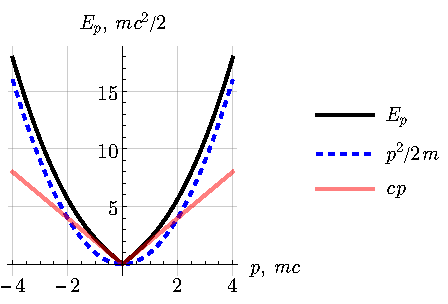
\includegraphics{imgs/MB71.pdf}
    \hspace{10 mm} 
    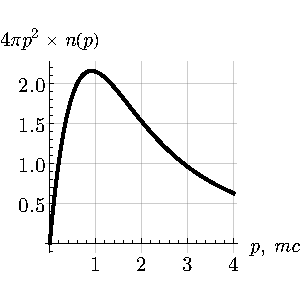
\includegraphics{imgs/MB72.pdf}
    \caption{Exitation energy $E_p$ and the momentum distribution function in 3D $4 \pi p^2 n(p)$}
    \label{fig:MB712}
\end{figure}


\textbf{4. Large canonical ensemble}. In zero order ($N_0 \approx N$) we have $\hat{H} - \mu \hat{N} = - \mu N + \frac{N^2}{2V}\varphi$, thus $\Omega_0 = \bk{\psi}[\hat{H}- \mu \hat{N}]{\psi} \to \min$ and 
\begin{equation*}
	\mu = \varphi n,
\end{equation*}
and we get $\Omega_0 = - \frac{N^2}{2V} \varphi$, so pressure is $P_0 = - \Omega_0 /V$ and hydrodynamic speed of sound
\begin{equation*}
	c^2 = \frac{\partial P_0}{\partial \rho} = V \frac{\partial }{\partial (m N)} \left(- \frac{\Omega_0}{V}\right) = \frac{n \varphi}{m},
\end{equation*}
so we could  rewrite $E_p$ as
\begin{equation}
	E_p = \sqrt{\left(\frac{p^2}{2m}\right)^2 + (cp)^2},
	\hspace{1cm} \Rightarrow \hspace{1cm}
	E_p = \left\{\begin{aligned}
	    &p^2 / 2m, &|p| \gg mc, \\
	    &c |p| , &|p| \ll mc.
	\end{aligned}\right.
\end{equation}
In the long-wave limit, the excitation spectrum has an acoustic character, and the calculated energy deviates from the linear law towards higher energies (fig. \ref{fig:MB712}).


\textbf{5. Ground state and compressibility}. Using \eqref{HBT} and \eqref{Ap} we could calculate the ground state energy
\begin{equation}
	\bk{0}[\hat{H} - \mu \hat{N}]{0} = \Omega_0 = - \mu N + \frac{N^2}{2V}\varphi +\frac{1}{2} \sum_{p \neq 0} (E_p - \epsilon_p).
	\label{BECgs}
\end{equation}
Yes, $\sum_{p \neq 0} (E_p - \epsilon_p)$ diverges as $E_p - \epsilon_p \approx - m n_0^2 \varphi^2 / p^2$ at $p \gg mc$, but for now we will ignore this and find 
\begin{equation*}
	\Omega_0 = - \frac{V}{2\varphi} \mu^2 - \sum_{p > 0} \left(
		\varepsilon_p + \mu - \sqrt{\varepsilon_p^2 - 2 \varepsilon_p \mu} 
	\right)
\end{equation*}
with $N = \mu V  / \varphi$, $n = \mu / \varphi$. Isothermal compressibility is equal
\begin{equation*}
	\kappa = - \frac{1}{V} \frac{\partial^2 \Omega}{\partial \mu^2} = \frac{1}{\varphi} + \frac{1}{V} \sum_{p > 0} \frac{\sqrt{\varepsilon_p}}{(\varepsilon_p -2\mu)^{3/2}},
	\hspace{0.5cm} \Rightarrow \hspace{0.5cm}
	\lim_{\varphi \to 0} \kappa = +\infty,
\end{equation*}
corresponding to the limit of the ideal Bose gase. 


% \textbf{Isothermal compressibility}. 